\section{Матрицы связности и достижимости в графе. Найти матрицу достижимости для указанного 
орграфа, с ее помощью выделить компоненты сильной связности графа.}

Пусть $A$ -- матрица смежности $G$, $|V|=n$. Найдем $B=E+A+A^2+ \dots +A^n$.

Определим матрицу $D$ размерности $n \times n$, $d_{ij}=sign(b_{ij})$.

Эта матрица показывает, есть ли путь из вершины $v_i$ в вершину $v_j$ (в этом
случае $d_{ij}=1$).

\begin{definition}
    В случае если граф $G$ -- неориентированный, матрица $D$
    называется матрицей связности. В случае, если граф $G$ -- ориентированный,
    матрица $D$ называется матрицей достижимости.
\end{definition}

Если $G$ -- неориентированный граф, $v_i \in V$, то в одну компоненту связности с
вершиной $v_i$ входят такие вершины $v_j$, для которых $d_{ij} = 1$.

Можно также ввести матрицу, по которой можно найти компоненты сильной
связности ориентированного графа.

Пусть $D$ -- матрица достижимости орграфа $G, L=D^T$,
\begin{align*}
    l_{ij}&=\begin{cases}
        1,& \text{если есть маршрут из $v_j$ в $v_i$},\\
        0,& \text{если нет}.
        \end{cases} \\
    F &= D \times L, f_{ij}=d_{ij} * l_{ij}.
\end{align*}
Если $f_{ij}$ = 1 , то вершины $v_i$ и $v_j$ принадлежат одной компоненте сильной
связности.

Пример. Рассмотрим ориентированный граф $G(V,E)$
\begin{figure}[h]
    \centering
    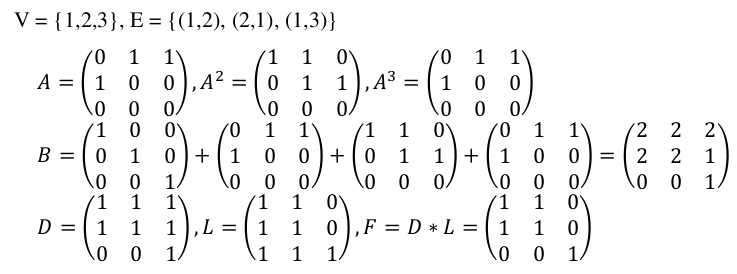
\includegraphics[scale=0.30]{18.png}
\end{figure}

Поэтому у графа 2 компоненты сильной связности $\set{1,2}$ и $\set{3}$.
Это один из способов нахождения компонент сильной связности. Временная
сложность $O(n^4)$.